\chapter{深度传感对照：共聚焦 / OCT / ToF}
\label{ch:09}

本章为选读。它不展开这些技术的全部细节，而是用前面各章的光学语言说明：它们各自靠什么获得深度，分辨率与量程由什么决定，以及与结构光、立体视觉的能力边界在哪里。

\section{效果}
\label{sec:ch09-effect}

读完本章，你应能：
\begin{enumerate}
  \item 说明共聚焦针孔如何实现光学层切，以及轴向分辨率与数值孔径的关系；
  \item 用第~\ref{ch:03}~章的相干长度解释 OCT 的轴向分辨率与量程；
  \item 区分脉冲 ToF 与相位（调幅连续波）ToF，写出相位 ToF 的距离公式与无模糊量程；
  \item 用一张对照表比较五类深度传感的分辨率、量程、对材料的敏感性与系统代价；
  \item 理解口内扫描常见选型背后的取舍。
\end{enumerate}

\section{原理}
\label{sec:ch09-principle}

\subsection{共聚焦：用针孔挑出焦面}

共聚焦系统把点光源聚焦到样品，再把返回光聚焦到与光源共轭的针孔上。焦面上的点回到针孔中心，全部通过；焦面外的点在针孔处是一个弥散斑，只有少部分通过。沿光轴扫描焦面（或扫描物体），记录每个横向位置的信号最大值所在深度，即得表面高度 \citep{WilsonSheppard1984}。

轴向响应宽度（层切厚度）近似
\begin{equation}
  \Delta z_{\mathrm{conf}}\sim\frac{\lambda}{\mathrm{NA}^2}
  \label{eq:ch09-conf}
\end{equation}
（常数因子依赖针孔大小与定义，量级为 $0.5$--$1.5$）。与第~\ref{ch:01}~章的景深同源：$\NA$ 越大，焦面外越快模糊，层切越薄。

要点：
\begin{itemize}
  \item 深度来自\emph{焦点位置}，不需要三角基线，因此可以在很窄的探头里工作，遮挡少（照明与观测同轴）。
  \item 量程由焦面扫描行程决定；精度由轴向响应宽度与 $\SNR$ 决定，峰值插值可达响应宽度的一小部分。
  \item 并行化：用针孔阵列或光栅图案配合深度扫描，可一次获得一片区域，代价是串扰与扫描时间。
  \item 半透明材料内部的散射光被针孔大量拒绝，这是共聚焦对次表面散射天然较鲁棒的原因。
\end{itemize}

\subsection{OCT：低相干干涉}

光学相干层析（OCT）把样品臂与参考臂的反射光在探测器上干涉 \citep{Huang1991OCT}。光源是宽带低相干光（第~\ref{ch:03}~章）：只有两臂光程差小于相干长度 $l_c$ 时才出现干涉条纹。因此干涉信号的包络定位了「样品中哪一深度的反射与参考臂等光程」。

对高斯谱、中心波长 $\lambda_0$、半高宽 $\Delta\lambda$ 的光源，轴向分辨率（空气中）为
\begin{equation}
  \Delta z_{\mathrm{OCT}}=\frac{2\ln2}{\pi}\,\frac{\lambda_0^{2}}{\Delta\lambda}.
  \label{eq:ch09-oct}
\end{equation}
例：$\lambda_0=840\,\mathrm{nm}$、$\Delta\lambda=50\,\mathrm{nm}$，$\Delta z\approx6.2\,\mu\mathrm{m}$；在折射率 $n$ 的介质中再除以 $n$。注意它与\emph{横向}分辨率解耦：横向由聚焦 $\NA$ 决定，轴向由光谱宽度决定。

\begin{itemize}
  \item \textbf{时域 OCT}：机械扫描参考臂长度。
  \item \textbf{频域 OCT}：参考臂固定，用光谱仪或扫频光源记录干涉光谱，傅里叶变换得到整条深度剖面。量程由光谱采样间隔决定，$z_{\max}\approx\lambda_0^2/(4\,\delta\lambda)$（$\delta\lambda$ 为每个光谱采样的宽度）。
\end{itemize}
OCT 的独特能力是\emph{看进去}：给出组织内部多层界面的反射，而不仅是表面。代价是量程浅（毫米级）、需要逐点或逐线扫描、系统复杂。

\subsection{ToF：飞行时间}

\textbf{脉冲 ToF}：发出短脉冲，测量往返时间 $\Delta t$，$Z=c\Delta t/2$。$1\,\mathrm{mm}$ 深度对应约 $6.7\,\mathrm{ps}$ 往返时间，可见毫米级精度需要皮秒级时间分辨。

\textbf{相位 ToF（调幅连续波）}：光源强度按调制频率 $F_m$（角频率 $\omega_m=2\pi F_m$；注意：$F_m$ 是强度包络的调制频率，通常为数十兆赫兹，远低于光频 $\nu$）正弦调制。返回光相对发射光有相位延迟 $\phi_m$，则
\begin{equation}
  Z=\frac{c}{4\pi F_m}\,\phi_m,\qquad Z_{\mathrm{amb}}=\frac{c}{2F_m}.
  \label{eq:ch09-tof}
\end{equation}
$Z_{\mathrm{amb}}$ 为无模糊量程：$F_m=20\,\mathrm{MHz}$ 时约 $7.5\,\mathrm{m}$。相位通常由每像素四个相位采样求得，形式与第~\ref{ch:06}~章的四步相移完全相同 \citep{LangeSeitz2001ToF}，于是深度噪声
\[
  \sigma_Z\approx\frac{c}{4\pi F_m}\,\sigma_{\phi_m},
\]
$\sigma_{\phi_m}$ 同样反比于调制幅与 $\SNR$。这里的「条纹」不在空间而在时间上：$c/(2F_m)$ 扮演条纹周期的角色。即便 $F_m=100\,\mathrm{MHz}$，周期也有 $1.5\,\mathrm{m}$，$0.01\,\mathrm{rad}$ 相位噪声对应约 $2.4\,\mathrm{mm}$。这解释了 ToF 在近距离精细测量上的根本劣势。多频 ToF 展开相位的思路与第~\ref{ch:06}~章多频外差相同。

ToF 的典型误差：多径干扰（墙角、凹面中光经过多次反射，等价于结构光的互反射）、次表面散射造成的延迟、混合像素（边缘飞点），以及温度引起的相位漂移。

\subsection{能力边界对照}

\begin{table}[htbp]
  \centering
  \small
  \begin{tabular}{@{}p{0.10\textwidth}p{0.12\textwidth}p{0.19\textwidth}p{0.19\textwidth}p{0.22\textwidth}@{}}
    \toprule
    方式 & 深度来源 & 轴向分辨率（量级） & 量程（量级） & 主要限制 \\
    \midrule
    共聚焦 & 焦点位置 & $1$--$20\,\mu\mathrm{m}$ & $0.1$--$20\,\mathrm{mm}$ & 扫描时间、$\NA$ 与视场 \\
    OCT & 相干门 & $2$--$10\,\mu\mathrm{m}$ & $0.5$--$5\,\mathrm{mm}$ & 量程浅、逐点扫描 \\
    结构光 & 三角+相位 & $3$--$50\,\mu\mathrm{m}$ & $1$--$500\,\mathrm{mm}$ & $\MTF$、散射、遮挡 \\
    立体 & 三角+匹配 & $10\,\mu\mathrm{m}$--$1\,\mathrm{mm}$ & $1\,\mathrm{mm}$--$20\,\mathrm{m}$ & 纹理、基线 \\
    ToF & 往返时间 & $1$--$30\,\mathrm{mm}$ & $0.1$--$20\,\mathrm{m}$ & 多径、时间分辨 \\
    \bottomrule
  \end{tabular}
  \caption{深度传感方式能力边界（数量级示意，非具体产品指标）。}
  \label{tab:ch09-compare}
\end{table}

图~\ref{fig:ch09-compare} 把同样的信息画在分辨率–量程平面上。可以看到一条大致规律：\emph{深度分辨率与量程之比}大体被各自的「编码尺度」锁定——共聚焦是焦深，OCT 是相干长度，结构光是条纹周期与基线，ToF 是调制周期。

\begin{figure}[htbp]
  \centering
  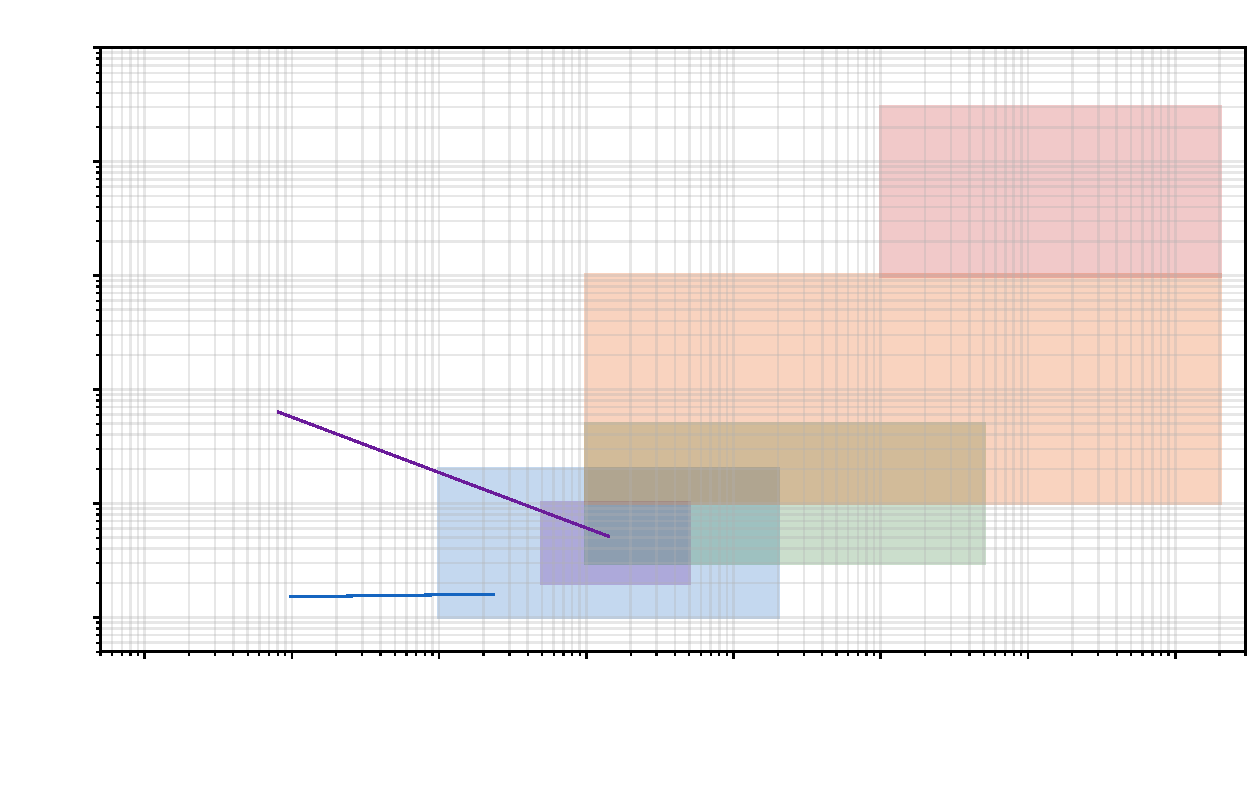
\includegraphics[width=0.85\textwidth]{fig-sensor-compare.pdf}
  \caption{各深度传感方式在分辨率–量程平面上的大致位置（概念草图，数量级示意）。}
  \label{fig:ch09-compare}
\end{figure}

\section{限度}
\label{sec:ch09-limits}

\begin{itemize}
  \item 式~\eqref{eq:ch09-conf}、\eqref{eq:ch09-oct} 的常数因子依赖定义（半高宽、针孔尺寸、谱形），只能做量级比较。
  \item 对照表忽略了速度、成本、体积与安全（激光功率）等维度，它们往往决定实际选型。
  \item 介质折射率改变光程：OCT 与 ToF 测得的是光程而非几何距离；半透明材料中共聚焦与结构光也会受到影响。
  \item 本章不涉及光度立体、焦点堆栈（depth from focus）等其他方法，它们与共聚焦或立体的原理相近。
\end{itemize}

\section{对象}
\label{sec:ch09-object}

\textbf{口内扫描常见选型（数量级示意）。} 口内场景的约束是：工作距十余毫米、深度范围数毫米到十余毫米、探头狭小、手持移动、表面湿润且半透明、精度目标数十微米。
\begin{itemize}
  \item \textbf{结构光}（相机+投影或多相机+条纹）：帧率高，单帧覆盖面积大，便于拼接；短板是散射与高反（第~\ref{ch:06}~章），以及基线受探头尺寸限制（第~\ref{ch:07}~章）。
  \item \textbf{并行共聚焦}：同轴、无遮挡、对散射较鲁棒，适合深窄的龈沟与邻面；但需要焦面扫描，单帧时间较长，对运动敏感，探头光学更复杂。
  \item \textbf{OCT}：能看到釉质下的结构（龋损、修复体界面），研究价值大；作为全牙弓表面扫描，量程与速度不足。
  \item \textbf{ToF}：精度远不够口内要求，主要见于房间尺度或人体尺度的测量。
\end{itemize}
不同产品的取舍差异主要在：用多少帧换精度、用什么方式对付散射与高反、探头允许的基线与景深。

\section*{本章收束}
共聚焦用焦点，OCT 用相干门，ToF 用往返时间，结构光与立体用三角。每种方法都有一个「编码尺度」，分辨率是这个尺度的一小部分，量程是它的若干倍。相位 ToF 与相移结构光在数学上同构，只是一个在时间上、一个在空间上编码。口内扫描以结构光与并行共聚焦为主，取舍落在速度、散射鲁棒性与探头尺寸上。

\section{习题}
\label{sec:ch09-exercises}

\begin{enumerate}
  \item \textbf{（计算）} 共聚焦物镜 $\NA=0.3$、$\lambda=488\,\mathrm{nm}$，估算层切厚度量级。若改为 $\NA=0.1$ 呢？对口内全牙扫描意味着什么？
  \item \textbf{（计算）} OCT 光源 $\lambda_0=1300\,\mathrm{nm}$、$\Delta\lambda=100\,\mathrm{nm}$，求空气中与牙釉质（$n\approx1.6$）中的轴向分辨率。
  \item \textbf{（计算）} 相位 ToF $F_m=60\,\mathrm{MHz}$，求无模糊量程；若相位噪声 $0.005\,\mathrm{rad}$，深度噪声多少？与口内精度目标对比。
  \item \textbf{（重建场景）} 在深而窄的龈沟中，结构光扫描缺失严重而共聚焦扫描较完整。从光路几何解释。
  \item \textbf{（重建场景）} ToF 相机拍摄墙角时，角落深度系统性偏大且角落被「磨圆」。原因是什么？它与结构光中的哪种误差同源？
  \item \textbf{（设计）} 若要检测修复体边缘下方的微小间隙（数十微米、位于表面下方），应考虑哪种方法？说明理由与代价。
\end{enumerate}

\section{习题讲解}
\label{sec:ch09-solutions}

\begin{enumerate}
  \item $\lambda/\NA^2\approx0.488/0.09\approx5.4\,\mu\mathrm{m}$；$\NA=0.1$ 时约 $49\,\mu\mathrm{m}$。$\NA$ 大层切薄、精度高，但视场与景深小，需要更长的扫描行程与时间；口内常取中等 $\NA$ 折中。
  \item $\Delta z=0.44\times1300^2/100\,\mathrm{nm}\approx7.5\,\mu\mathrm{m}$（空气），釉质中约 $4.7\,\mu\mathrm{m}$。
  \item $Z_{\mathrm{amb}}=c/(2F_m)=2.5\,\mathrm{m}$；$\sigma_Z=c\sigma_{\phi_m}/(4\pi F_m)\approx3\times10^8\times0.005/(4\pi\times6\times10^7)\approx2\,\mathrm{mm}$，比口内目标大约两个数量级。
  \item 结构光需要投影与相机两个方向都能看到沟底，基线带来阴影与遮挡；共聚焦照明与观测同轴，只要一个方向能看到即可。
  \item 多径干扰：光在两面墙之间多次反射后返回，路径更长，相位延迟偏大。与结构光中的互反射同源，都违反「每像素只接收一次直接反射」的假设。
  \item OCT：能分辨表面以下的界面，轴向分辨率数微米。代价：量程浅、扫描慢、系统复杂，需与表面扫描配合使用。
\end{enumerate}
